While the previous chapter provides an architecture within which transport and network layers exchange relevant information, it does not define how networks should select outgoing paths. 
This chapter presents a possible solution for balancing traffic according to expected congestion which works under a wide range of network conditions.

\section{A model for congestion balancing}

%2.2) Mathematical detail of balancing equation -- motivate
% parameterisedequation with equal share vs conservative vs loss-based
Consider \ac{LEX}-capable traffic, that is explicitly marked as either being retransmitted or non-retransmitted, from a single origin prefix to a single destination prefix, with a number of possible paths and within a single time period.  
Let $N$ be the number of paths (numbered $1,\ldots,N$). 
Let $T_i$ be the number of bytes sent down path $i$ for the previous time period. 
Let $R_i$ be the number of bytes marked as retransmissions down path $i$ for the previous time period.  
Let $R=\sum_i R_i$ and $T=\sum_i T_i$.
While $R_i$ does not strictly represent the number of lost bytes, the ratio of $R_i/T_i$ should be a good approximation of the loss rate within period $i$.
A starting assumption is that it is desirable to equalise the proportion of lost bytes on all paths -- that is make $R_i/T_i$ equal for all $i$ -- since doing so maximizes social welfare and mimics the behaviour of existing end-host only resource pooling solutions such as \ac{MPTCP}.

The loss rate $\rho_i = R_i/T_i$ to be balanced is an unknown function of $T_i$ and $B_i$ the bandwidth of the link.
It is, however, likely that the loss rate is increasing or at least non-decreasing with $T_i$.
Similarly, the loss rate is decreasing or at least non-increasing with the unknown $B_i$.
Assume then that whatever the true function, for a small region around the current values of $T_i$ and $B_i$ then it is locally linear $\rho_i = k_i T_i/B_i$ where $k_i$ is an unknown constant.
Substituting gives
\begin{equation}
B_i/k_i = T_i^2/R_i.
\label{eqn:bik}
\end{equation}

Now consider the next time period.  
Use the dash notation for the same quantities in the next time period.  
In typical time periods $\E{T'} = \E{T}$ since, for example, if the next time period on average had more traffic, the overall amount of traffic would be growing. 
While this is true in the year-on-year setting, this effect is negligible in the time scale discussed here.
Now $\rho'_i = R'_i/T'_i = k T'_i/B'_i$.  
Choose the $T'_i$ to make all $R'_i/T'_i = C$ (hence all equal) where $C$ is some unknown constant.  
Therefore $T'_i = C B'_i/k'_i$ but if this is still near the locally linear region then $B'_i/k'_i \simeq B_i/k_i$ and $B_i/k_i$ is determined by \eqref{eqn:bik} hence the predicted distribution is $ T'_i = C T_i^2/R_i$.  
Now it is necessary to calculate $C$ by summing over $i$.  
$T = C \sum_i T_i^2/R_i$ and hence $C = T/\sum_i T_i^2/R_i$.
This results in a usable loss balancing equation given the available system inputs:

\begin{equation}
T'_i = \frac{T T_i^2}{R_i \sum_j (T_j^2/R_j)}.
\label{eqn:routesplitloss}
\end{equation}

There is, of course, a problem when $R_i = 0$.  
Given the assumption that the traffic is assigned in inverse proportion to loss rate, a branch with no loss would naturally have all traffic assigned to it. 
To correct this, $R_i$ is incremented for each path by one \ac{MSS}. 
This problem is further explored in subsequent sections.

\subsection{Understanding the design space}

\begin{figure}
    \begin{subfigure}[b]{.5\linewidth}
        \centering
        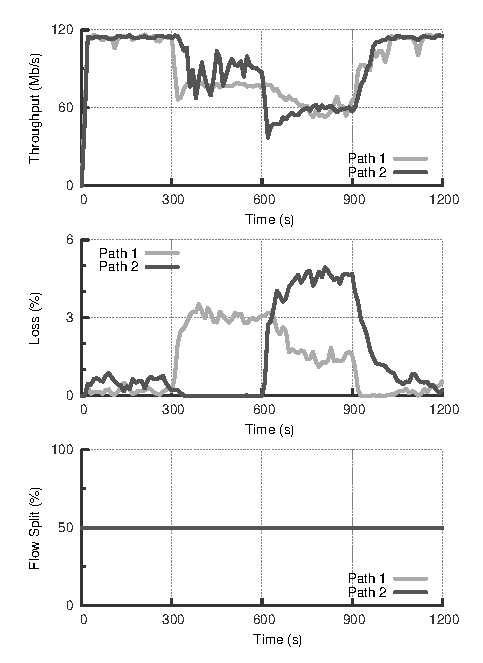
\includegraphics[width=2.5in]{figures/cate/two/equal}
        \caption{Equalisation.}\label{fig:twoequal}
    \end{subfigure}%
    \begin{subfigure}[b]{.5\linewidth}
        \centering
        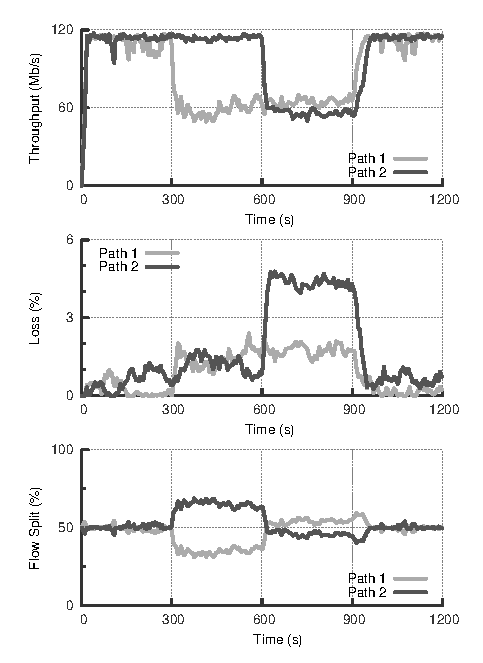
\includegraphics[width=2.5in]{figures/cate/two/cons}
        \caption{Conservative.}\label{fig:twocons}
    \end{subfigure}%

    \vspace{10mm}

    \begin{subfigure}[b]{.5\linewidth}
        \centering
        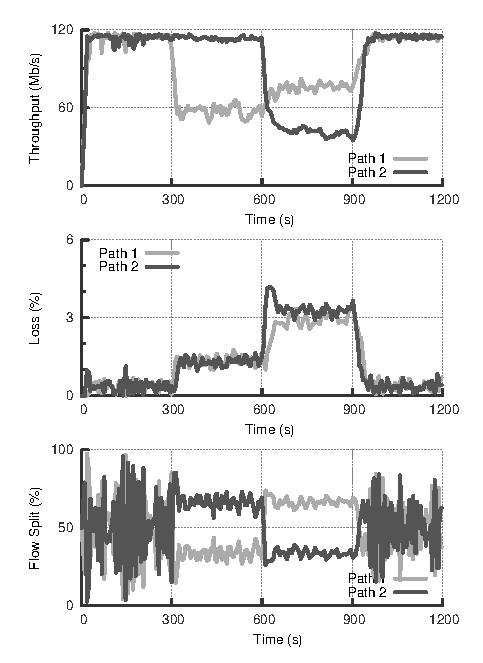
\includegraphics[width=2.5in]{figures/cate/two/loss}
        \caption{Loss-driven.}\label{fig:twoloss}
    \end{subfigure}%
    \begin{subfigure}[b]{.5\linewidth}
        \centering
        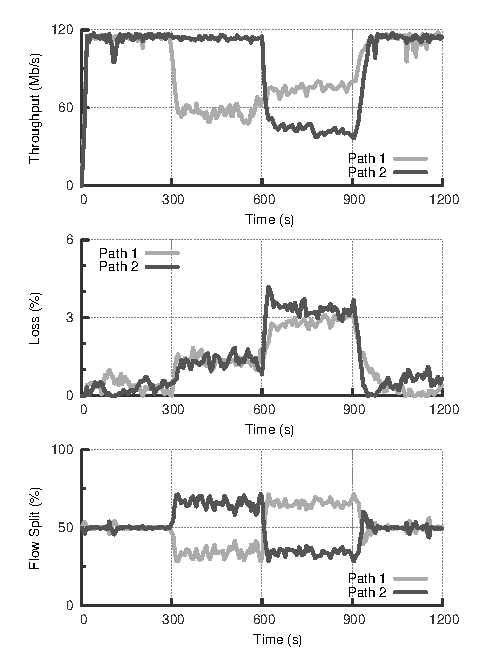
\includegraphics[width=2.5in]{figures/cate/two/correct}
        \caption{Balanced.}\label{fig:twopreflex}
    \end{subfigure}%

    \caption[Simulation using \acs{PREFLEX} to balance traffic over two paths.]
    {Simulation using \acs{PREFLEX} to balance traffic over two paths. \label{fig:two}
        Each simulation demonstrates the dynamics of a single mode, except for
        (\subref{fig:twopreflex}) which balances between conservative and loss-driven components.  }
\end{figure}

Given local linearity is assumed, large adjustments to the traffic split are a potential cause for concern.
Some traffic must also be assigned to each route independently of the loss rate, in order to probe whether the path is available.
This leads to a small component of equalisation being used to ascertain that paths are continually used.
Finally, in the absence of loss, it is practical to assign traffic according to the current traffic throughput split.  
This denotes a conservative approach to splitting traffic.
Therefore, there are three tendencies which must be accounted for: the loss-equalisation tendency from \eqref{eqn:routesplitloss}, the equalisation tendency to ensure some degree of utilization across all paths, and a conservative tendency to keep the traffic split the same as the throughput split in the previous period.
Call the traffic split assigned to path $i$  by each of these schemes $T(E)_i$, $T(C)_i$ and $T(L)_i$ where $E$, $C$ and $L$ stand for ``equal", ``conservative" and ``loss-driven".

The final distribution of traffic across all links is then:
$$
T'_i = \beta_E T'(E)_i + \beta_C T'(C)_i + \beta_L T'(L)_i,
$$
where the $\beta_\bullet$ are user set parameters in $(0,1)$ such that $\beta_E+\beta_C + \beta_L = 1$.  Now $T'(C)_i = T_i$ and $T'(E)_i = T/N$ where $N$ is the number of interfaces. 
This gives a first equation for the desired flow split $f'_i$, which represents the probability with which path $i$ will be assigned to a new flow:
\begin{equation}
f'_i = \frac{T'_i}{T} =  \beta_E \frac{1}{N} + \beta_C \frac{T_i}{T} +
\beta_L \frac{T_i^2}{R_i \sum_j (T_j^2/R_j)}.
\label{eqn:Tdashi}
\end{equation}


While \eqref{eqn:Tdashi} describes a very broad design space, intuition on how each component performs is provided through a simple example, which is described in full in section \ref{section:methodology}. 
Consider a network balancing traffic to a given prefix between two paths with equal bottleneck capacity $L_1=L_2=120$Mbps.
For reference, this topology is illustrated in figure \ref{fig:topo}.
For the duration of the experiment, a source balances traffic to $C$ through either link.
At $t=300$s, cross-traffic is generated from server $D_1$ towards client $C$ through $L_1$.
At $t=600$s, a greater quantity cross-traffic is generated from server $D_2$ towards client $C$ through $L_2$.
The respective throughput, loss rate and the proportion of flows assigned to each path are shown in figure \ref{fig:two} for cases where each component is used in isolation, and a final case in which all three components are balanced.

The effect of equalisation is the first to be considered, given it is necessary to ensure all paths are continually probed. 
Equalisation alone however leads to an inefficient use of the network if there is a mismatch in path capacity, as made apparent in figure \ref{fig:twoequal} as congestion occurs on either link. 
Such behaviour arises in traditional traffic engineering, which resorts to equalising traffic weighted by local link capacity.  
Where a bottleneck is remote and distinct however, such behaviour will lead traffic across all links to be roughly bound by the capacity of the slowest path, as can be seen between $t=300$s and $t=600$s where throughput over the first path is dragged down by congestion on a second path.  
Figure \ref{fig:twocons} and \ref{fig:twoloss} on the other hand show distinctive behaviour when using a solely conservative or solely loss-driven approach. 
Predictably for small values of loss the loss-driven approach overreacts and flaps between either path. 
While the net effect of these oscillations does not result in significant losses, a conservative approach lends itself more naturally to situations where loss is too small to provide a reliable indicator on path quality. 
Once loss becomes significant however a conservative approach is unable to drive traffic in order to balance loss across both paths. 
More worryingly, a pure conservative approach demonstrates the wrong dynamics, as highlighted between $t=250$s and $t=300$s. 
Despite being saturated, the balancer continues to push more traffic towards path 1 while the second path remains under-utilized, dropping its throughput further.

Note that in figure \ref{fig:two} the conservative approach obtains higher throughput than its loss-driven counterpart once loss settles in. 
While this may seem advantageous, in reality this behaviour will be shown to be detrimental to the system as a whole: only by balancing loss can social welfare be optimized \cite{Kelly:2005p140}.

\subsection{Balancing between conservative and loss-driven}

Ideally the proposed balancer should adjust between conservative and loss-driven modes for differing regimes of loss.
Equalisation is required in some measure as every path must attract some traffic if it is not to fall out of use (\cite{Kelly:2005p140}, remark 2). 
If this were not the case, a path with relatively high loss would never be probed to determine whether congestion has subsided.
The remaining two components must be balanced to be able to respond adequately to loss while not being overly sensitive to statistically insignificant fluctuations in loss. 
Let $\gamma$ replace both $\beta_C$ and $\beta_L$ in \eqref{eqn:Tdashi} and adjust between conservative and loss-driven modes:
\begin{equation}
f'_i = \beta_E \frac{1}{N} + \left( 1-\beta_E \right) \left(
\gamma \frac{T_i}{T} + \left(1-\gamma\right) \frac{T_i^2}{R_i \sum_j
(T_j^2/R_j)} \right).
\label{eqn:gamma}
\end{equation}

As a result, $\beta_E$ may now vary between $[0,1]$. 
A simple but effective value for $\gamma$ is to define a minimum average loss $\mu_{min}$ below which there loss is tolerated, and react increasingly as the average loss $\mu$ becomes more significant:
\begin{equation}
\gamma = 
\begin{cases} 
\frac{\mu_{min}}{\mu}, & \mbox{if }\mu > \mu_{min}\\
1, & \mbox{if }\mu \leq \mu_{min}
\end{cases}
\end{equation}

This completes the \ac{PREFLEX} balancer, as shown in figure \ref{fig:twopreflex}. 
The evolution of $\gamma$ for the example shown in figure \ref{fig:twopreflex} is shown in figure \ref{fig:tune}(left). 
The value of $\mu_{min}$ was set to $0.005$.

\begin{figure}
    \centering
    \begin{subfigure}[b]{.5\linewidth}
        \centering
        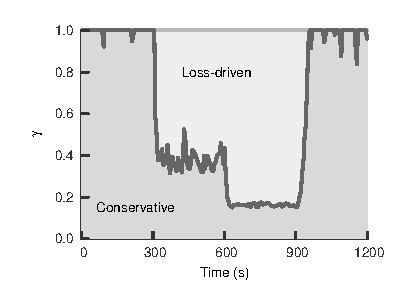
\includegraphics[width=0.9\linewidth]{figures/cate/gamma}
        \caption{$\gamma$ \label{fig:gamma}.}
    \end{subfigure}%
    \begin{subfigure}[b]{.5\linewidth}
        \centering
        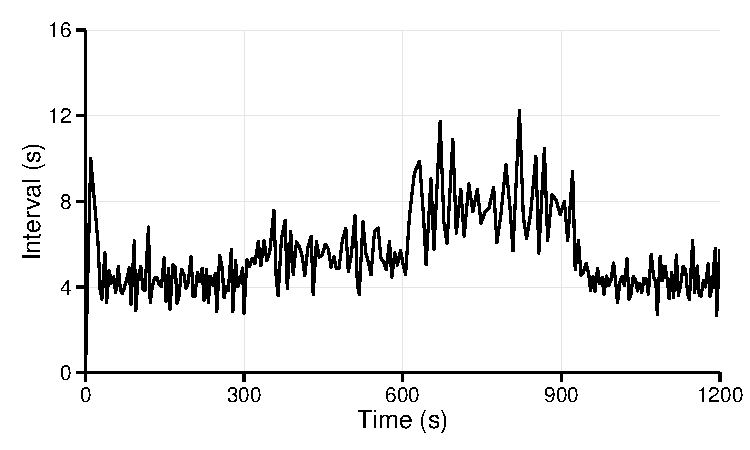
\includegraphics[width=0.9\linewidth]{figures/cate/tau}
        \caption{$\tau'$ \label{fig:tau}.}
    \end{subfigure}
    \caption[Parameters $\gamma$ and $\tau'$]{Self-tuning parameters for example in figure \ref{fig:twopreflex}.}
    \label{fig:tune}
\end{figure}

\subsection{Tuning update interval}
%2.3) Automatic parameter tuning -- describe tuning of timescales and
% of parameters for 2.2.  Perhaps include diagram showing different
% regime where different parameters are needed (e.g. equal traffic on
% all pathsprobes unused paths, conservative works in low loss regime,
% loss-basedworks in high loss regime).
A further potential issue is how often the flow split should be updated considering the sparseness of loss.
Assume that for a given prefix packet loss is measured over a given time period $\tau$.  
It would be practical to tune this $\tau$ per prefix according to the accuracy afforded by the loss estimate.
If $\tau$ is short then only a very small number of packets will be lost. 
On the other hand, if $\tau$ is long then the control system will be unable to react quickly to changes.  
$\tau$ should therefore be sufficiently small that an accurate measure of loss can be obtained.  
As a result, it is useful to have a rough estimate of the measurement period required to ensure accurate loss estimates.
Since this time period of measurement is per prefix, this must to some extent reflect the importance a given measurement to the system as a whole.
For example, the overall system should not be held up by a single route with insufficient traffic for an accurate measurement to be obtained.
This will be achieved with the concept of a weighted coefficient of variation.

Let $t_i$ be the number of packets transmitted down path $i$ in the time period $\tau$ and let $l_i$ be the number of packets which were lost in this time period.
To prevent the aforementioned divide by zero issue, $l_i = 1\ac{MSS}$ if no packets are lost.

Let $p_i$ be the probability that a given packet is lost on path $i$ and assume that packet loss is a Bernoulli process.  
An unbiased estimate of $p_i$ is $\hat{p_i} = l_i/t_i$.
It is important to what follows that $\hat{p_i}$ is only an estimate of $p_i$ by ``chance" more or fewer packets may have been lost.
Given packet loss is Bernoulli then $l_i$ has a binomial distribution and its variance $\sigma^2$ is given by $t_i p(1-p)$.  
The \ac{CV}, is a dimensionless measure given by the standard deviation over the mean $c_v= \sigma/\mu$.  
Keeping the coefficient of variation within some bound $\delta$ is a measure of the amount by which an estimate is likely to vary from the true mean.

From trivial definitions of $\sigma$ and $\mu$, for the number of lost packets on a given prefix $i$ the estimated \ac{CV} is $\hat{c_v(i)} = \sqrt{t_i \hat{p_i}(1- \hat{p_i})}/t_i\hat{p_i}$.
Let $r_i$ be the rate of packet arrival per unit time on $i$ giving $t_i= r_i \tau$.  
Define $W$ the \ac{CV} weighted by transmitted packets over the prefix as $W= \sum_i t_i/t \hat{c_v(i)}$ where $t= \sum_i t_i$ and this expands as $$W =  \sum_i \frac{t_i}{t} \sqrt{\frac{ (1- \hat{p_i})} {r_i \tau }}.$$

The ``accuracy" of the measurement of $p_i$ is determined by the accuracy of $l_i$ and hence, for the prefix as a whole by the \ac{CV} $W$.
The aim now is to pick the time period for the next measurement $\tau'$ such that $W \leq \delta$ for some $\delta$.  
Assuming that the loss rates and traffic rates will be the same in the next time period will give a good indication of how to set $\tau'$.  
Therefore for the next time period $$\delta \geq W = \frac{1}{\sqrt{\tau'}}\sum_i \frac{t_i}{t} \sqrt{\frac{(1- \hat{p_i})} {r_i }}.$$
This gives an estimated minimum time period to set for the next time period. 
In order to get weighted \ac{CV} of packet loss (and hence loss rate) equal to or below $\delta$ the time period $\tau'$ is bounded by
$$
\tau' \geq \tau \left( \frac{1}{\delta t}\sum_i
\sqrt{t_i- l_i} \right)^2.
$$
This equation gives the smallest value to set the time period of measurement to in order that the weighted coefficient of variation of the loss measurement is a given $\delta$. An upper bound for this value should be set by operators to ensure that the system periodically updates flow splits when operating under extremely low loss rates.
    
While a number of simplifying assumptions have been made, such as modelling loss as Bernoulli, the time scale choice is not a critical system parameter so long as it provides ``good enough" estimates of loss. 
The evolution of $\tau'$ for the example in figure \ref{fig:twopreflex} is plotted in figure \ref{fig:tune}. 
As throughput decreases, the time between updates is inflated to adjust to the lower occurrence of loss events. 
